\documentclass{beamer}
 
\usepackage[utf8]{inputenc}
\usepackage[italian]{babel}
\usepackage[T1]{fontenc}
\usepackage{setspace}
 
\usetheme{Madrid} 

%Information to be included in the title page:
\titlegraphic{
\includegraphics[width=1.8cm]{unitn.png}
}
\title[Laurea in Informatica]{Identifying and Classifying Symptoms\\within a Patient's Statement}
\author{Nicola Sartorato}
\institute[UNITN]{Universitá di Trento}
\date{23 settembre 2019}

 
\begin{document}

\frame{\titlepage}

\setstretch{1.20}

\begin{frame}
\frametitle{Indice}

\begin{itemize}
\setlength\itemsep{1em}
\item Il problema e le motivazioni
\item La soluzione
\end{itemize}

\end{frame}
 
\begin{frame}
\frametitle{Il macro-obiettivo}

\begin{block}{Il macro-obiettivo}
Sviluppare un agente conversazionale capace di condurre l'\textbf{anamnesi} sostituendosi al medico.
\end{block}

\pause

\begin{alertblock}{L'anamnesi}
È la raccolta dalla voce diretta del paziente di tutte le informazioni utili al medico per effettuare una diagnosi.
\end{alertblock}

\end{frame}

\begin{frame}
\frametitle{Il problema e le motivazioni}
I medici, infatti:

\begin{itemize}
 \item<1-> svolgono il loro lavoro sotto stringenti \textbf{limitazioni di tempo} \pause
 \item<2-> sono occupati principalmente da \textbf{lavori di scrivania }(49.2\% del loro tempo) e solo il 27\% del loro tempo sono a contatto con i pazienti \pause
 \item<3-> l'attività per loro più intensa è l'\textbf{anamnesi}, la quale è:
 \begin{enumerate}

  \item<1-> \textbf{fondamentale}\pause
  \item<2-> ma a volte \textbf{incompleta}
 \end{enumerate}
\end{itemize}

\end{frame}

\begin{frame}
\frametitle{A piccoli passi}

\begin{block}{Il primo ostacolo}
\textbf{Identificare} e \textbf{classificare} i sintomi all'interno di una frase detta da un paziente.
\end{block} \pause

\begin{exampleblock}{Identificare un sintomo}
Individuare all'interno di una frase ogni gruppo di parole adiacenti che, insieme, vogliono dire un sintomo.
\end{exampleblock}\pause

\begin{exampleblock}{Classificare un sintomo}
Mappare i sintomi precedentemente identificati in sintomi specifici che fanno riferimento ad una classificazione.
\end{exampleblock}

\end{frame}

\begin{frame}
\frametitle{Identificare un sintomo}

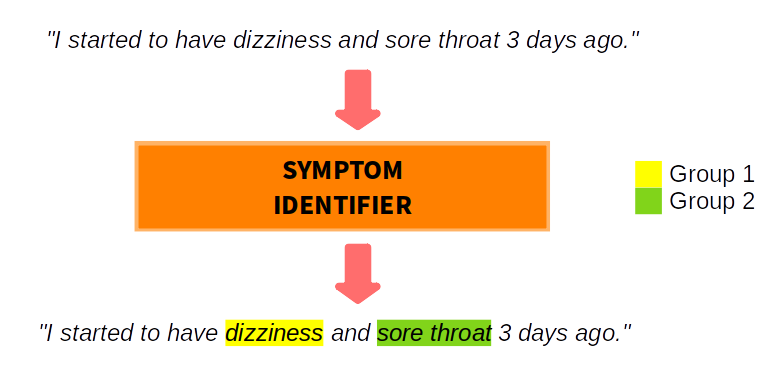
\includegraphics[width=\textwidth]{images/symptom_identifier.png}

Il \textbf{Symptom Identifier} riceve in input la frase del paziente e restituisce i sintomi identificati (i \emph{tokens for predictions}).

\end{frame}

\begin{frame}
\frametitle{Classificare un sintomo}

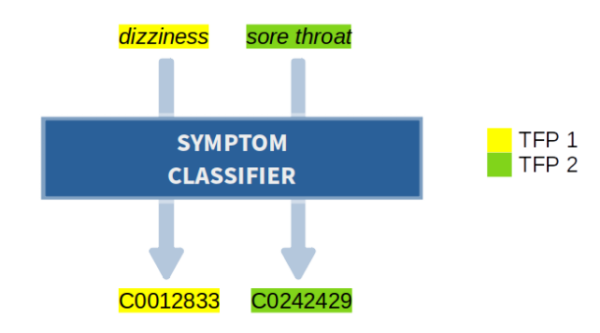
\includegraphics[width=\textwidth]{images/symptom_classifier1.png}

Il \textbf{Symptom Classifier} riceve in input i \emph{tokens for predictions} e restituisce i codici univoci dei sintomi identificati (i CUIs).

\end{frame}

\begin{frame}
\frametitle{La classificazione di sintomi}

La classificazione di sintomi utilizzata è MEDCIN:
\begin{itemize}
  \item si trova all'interno dei dizionari supportati da UMLS (Unified Medical Language System), che fornisce un CUI (Concept Unique Identifier) per ogni suo termine
  \item ha un'organizzazione gerarchica (i.e. ad albero)
\end{itemize}


\end{frame}

\begin{frame}
\frametitle{Metodi: il Symptom Identifier}
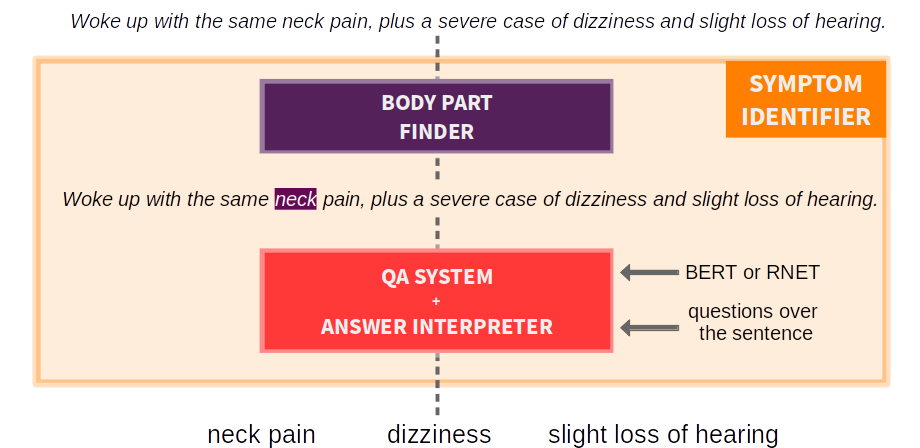
\includegraphics[width=\textwidth]{images/methods_overview1.png}
\end{frame}

\begin{frame}
\frametitle{Metodi: il Symptom Identifier}
Il \textbf{Symptom Identifier} è composto da tre componenti:\pause
\begin{enumerate}
 \item dal \textbf{Body Part Finder} che evidenzia le parti del corpo all'interno della frase\pause
 \item dal \textbf{Question Answering System } che si occupa di estrarre, usando Machine Reading Comprehension, il problema generico del paziente e quelli delle parti del corpo presenti nella frase. Lo fa sfruttando uno di questi due modelli:\pause
  \begin{itemize}
    \item BERT (Devlin, 2018) è un modello pretrained che consente \pause
    \item R-NET
  \end{itemize}
\end{enumerate}
\end{frame}

\begin{frame}
\frametitle{Metodi: il Symptom Identifier}
\begin{enumerate}
 \setcounter{enumi}{2}
  \item dall'\textbf{Answer Interpreter}
\end{enumerate}
\end{frame}

\begin{frame}
\frametitle{Metodi: il Symptom Classifier}
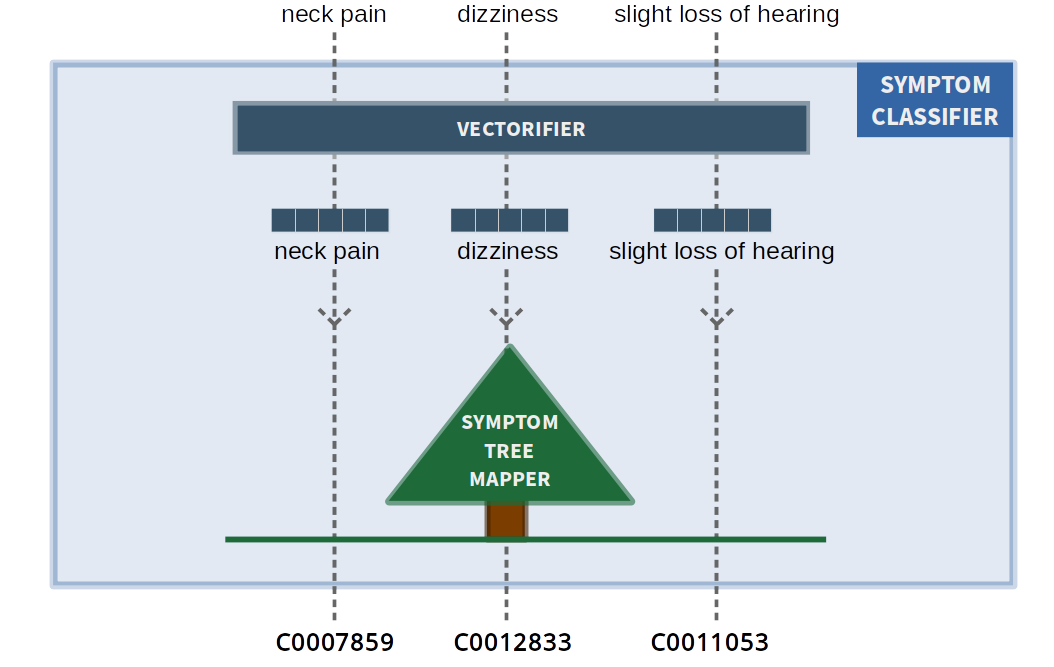
\includegraphics[width=\textwidth]{images/methods_overview2.png}
\end{frame}

\begin{frame}
\frametitle{Metodi: il Symptom Classifier}
Il Symptom Classifier :
\begin{itemize}
 \item ..
\end{itemize}
\end{frame}

\end{document}
